\chapter{Организация параллельных вычислений в модели мелкой воды}\label{ch:ch2}

\section{Программная архитектура модели}\label{sec:ch2/sec1}

Программная архитектура играет ключевую роль в климатических моделях, и в частности в моделях океана.
Способность модели эффективно работать на различных вычислительных системах во многом зависит от выбора правильной программной архитектуры, которая должна обеспечивать гибкость, масштабируемость и переносимость модели на различные типы вычислительных систем.
Помимо этого, гибкая программная архитектура существенно упрощает интеграцию новых компонентов и алгоритмов, что крайне важно при разработке модели.

В данной работе, для модели мелкой воды была реализована программная архитектура, основанная на принципе разделения обязанностей.
Программная архитектура заключается в том, что весь программный комплекс разделяется на три уровня: самый нижний уровень, уровень Ядра, содержит все процедуры, необходимые для вычисления уравнений мелкой воды, так называемые ядра модели; самый высокий уровень, уровень Алгоритма, отвечает за порядок вызова ядер модели и задает схему работы модели по времени; уровень Интерфейса выступает в качестве промежуточного уровня между первыми двумя и отвечает за параллельные методы и подходы, используемые в модели. 
Программные архитектуры такого типа позволяют выделить параллельные методы в обособленную часть программы (уровень Интерфейса) с целью их адаптации и гибкой настройки на целевую вычислительную систему. Причем это делается без изменений частей программы, отвечающих за вычисления уравнений мелкой воды.
Выделение параллельного ядра в отдельную часть программы также существенно упрощает разработку, отладку и оптимизацию кода под целевую вычислительную систему.

Трехуровневая программная архитектура, основанная на принципе разделения обязанностей, успешно зарекомендовала себя в модели океана NEMO (Nucleus for European Modeling of the Ocean) \cite{gmd-11-3447-2018}. 
%Исследователи планируют реализовать такую программную архитектуру во всей модели океана NEMO к 2022 году [15].

Как уже упоминалось ранее, модель полностью написана на языке Fortran, что оказывает существенное влияние на программную архитектуру и ее реализацию.
В программном коде модели широко используются модули, производные типы (классы), интерфейсы и макросы.
Отметим, что программный код для графических процессоров написан с использованием синтаксиса CUDA Fortran. 
Опишем каждый уровень программной архитектуры модели более подробно.

\subsection{Уровень Ядра}

Уровень Ядра содержит все вычислительные подпрограммы, так называемые ядра модели. Исходная непараллельная программа представляет собой набор именно таких подпрограмм.
Всего в модели мелкой воды насчитывается около 15 ядер. Ядро модели представляет собой подпрограмму, в которой производятся вычисления сеточных переменный внутри некоторой заданной расчетной области. Важно отметить, что ядро модели не содержит программного кода, отвечающего за синхронизацию данных.
Это означает, что если подпрограмма имеет несколько расчетных циклов по точкам сетки и содержит синхронизацию данных между циклами, то такая подпрограмма должна быть разбита на несколько подпрограмм (ядер модели) без синхронизации данных.
За синхронизацию данных между вызовами ядер модели отвечает уровень Интерфейса, который будет рассмотрен позже.

В случае использования процессора (CPU) для вычислений, ядро модели представляет собой двумерный цикл по точкам сетки, в котором происходит обновление значений в каждой точке сетки с использованием численных схем.
На данном уровне происходит работа с обычными двумерными массивами.
На рис. \ref{fig:kernel}а) показан общий вид ядра модели для расчета на CPU, где nx\_start, nx\_end, ny\_start, ny\_end - границы подобласти; bnd\_x1, bnd\_x2, bnd\_y1, bnd\_y2 - границы подобласти, включая внерасчетные границы; var - сеточная переменная.

\begin{figure}[!ht]
	\begin{minipage}{\linewidth}
		\centering
		\begin{lstlisting}
subroutine kernel(var)
	real(wp8), intent(inout) :: var(bnd_x1:bnd_x2, bnd_y1:bnd_y2)
	[...]
	do m = nx_start, nx_end
		do n = ny_start, ny_end
			var(m, n) = [...]
		enddo
	enddo
end subroutine
		\end{lstlisting}
		\subcaption{Программный код для расчета на CPU}
	\end{minipage}
	\begin{minipage}{\linewidth}
		\centering
		\begin{lstlisting}
attributes(global) subroutine kernel(var)
	real(wp8), intent(inout) :: var(bnd_x1:bnd_x2, bnd_y1:bnd_y2)
	[...]
	m = (blockIdx%x-1)*blockDim%x + threadIdx%x + (nx_start - 1) - 1
	n = (blockIdx%y-1)*blockDim%y + threadIdx%y + (ny_start - 1) - 1
	if (m <= nx_end + 1 .and. n <= ny_end + 1) then
		var(m, n) = [...]
	endif
end subroutine
		\end{lstlisting}
		\subcaption{Программный код для расчета на GPU}
	\end{minipage}
	\vspace{3pt}
	\caption{Уровень Ядра модели мелкой воды}
	\label{fig:kernel}
\end{figure}

В случае использования графических процессоров (GPU) для вычислений, ядро модели обновляет значения в одной точке сетки в отличие от двумерного цикла по точкам сетки при вычислениях на CPU.
Каждой точке сетки соответствует свой поток на GPU, в котором производятся вычисления.
Запуск ядра модели на GPU осуществляется потоками, охватывающими все точки расчетной области. На рис. \ref{fig:kernel}б) показан общий вид ядра модели ядра для расчета на графических процессорах.

Таким образом, в данной работе было реализовано 15 ядер модели для расчетов уравнений мелкой воды как на CPU, так и на GPU.

\subsection{Уровень Алгоритма}

На самом верхнем уровне архитектуры программного обеспечения - уровне Алгоритма - определяется порядок вызова ядер и описывается основной временной цикл модели. На этом уровне работа ведется с абстрактными структурами данных, такими как класс ocean\_type, который содержит основные сеточные переменные для уравнений мелкой воды: уровень моря, компоненты скорости, и т.д.

Пример кода этого уровня представлен на рис. \ref{fig:algorithm}. В данном примере сначала вызывается ядро для расчета уровня моря (kernel\_ssh), а затем - ядро для расчета компонент скорости (kernel\_uv). Для вызова модельных ядер используется специальная процедура envoke, являющаяся частью уровня Интерфейса, и которая будет рассмотрена далее.

\begin{figure}[!ht]
	\centering
	\begin{lstlisting}
[...]
type(ocean_type), target :: ocean_data
procedure(empty_kernel), pointer :: kernel_ssh, kernel_uv
[...]
call envoke(ocean_data%ssh, kernel_ssh)
call envoke(ocean_data%u, ocean_data%v, kernel_uv)
[...]
	\end{lstlisting}
	\vspace{3pt}
	\caption{Уровень Алгоритма модели мелкой воды}
	\label{fig:algorithm}
\end{figure}

\subsection{Уровень Интерфейса}

\begin{figure}[!ht]
	\begin{minipage}{\linewidth}в
		\centering
		\begin{lstlisting}
subroutine envoke(var, kernel)
	type(data2D_real8_type) :: var
	[...]
	!$omp do private(k) schedule(static, 1)
	do k = 1, blocks
		call kernel(var%block(k)%host)
	enddo
	!$omp end do nowait
	call sync_halo
end subroutine
		\end{lstlisting}
		\subcaption{Интерфейс для запуска расчетов на CPU}
	\end{minipage}
	\begin{minipage}{\linewidth}
		\centering
		\begin{lstlisting}
subroutine envoke(var, kernel)
	type(data2D_real8_type) :: var
	[...]
	!$omp do private(k) schedule(static, 1)
	do k = 1, blocks
		cudaSetDevice(k-1)
		call kernel<<<tGrid, tBlock>>> (var%block(k)%device)
	enddo
	!$omp end do nowait
	call copy_device_to_host	
	call sync_halo
	call copy_host_to_device
end subroutine
		\end{lstlisting}
		\subcaption{Интерфейс для запуска расчетов на GPU}
	\end{minipage}
	\vspace{3pt}
	\caption{Уровень Интерфейса модели мелкой воды}
	\label{fig:interface}
\end{figure}

Промежуточным уровнем между ядром модели и вызовом ядра модели является уровень Интерфейса, на котором реализуются все параллельные методы и подходы в модели.
В частности, на этом уровне реализуются блочная декомпозиция (раздел \ref{sec:ch2/sec2}), метод балансировки нагрузки (раздел \ref{sec:ch2/sec3}), гибридный подход с использованием технологий MPI и OpenMP (раздел \ref{sec:ch2/sec4}), гибридные подходы с использованием технологий MPI, OpenMP и CUDA (раздел \ref{sec:ch2/sec5}) реализованы на уровне Интерфейса.
Уровень Интерфейса также включает программный код для синхронизации данных между процессорами, обмена данными с внерасчетными границами и передачи данных между CPU и GPU. Уровень Ядра и уровень Алгоритма содержат описание физических процессов в модели мелкой воды - однако на этих программных уровнях ничего неизвестно о деталях параллельной реализации, которые скрыты на уровне Интерфейса. Интерфейс позволяет гибко конфигурировать и настраивать модель для различных целевых вычислительных систем без изменения программного кода на уровнях Ядра и Алгоритма.
На уровне Интерфейса происходит работа со специальными типами данных, например, с классом типа data\_2D\_real\_8", который содержит распределенные по блокам и процессорам данные. В случае использования GPU такие типы данных дублируют данные в глобальной памяти GPU, а также содержат процедуры синхронизации этих данных между CPU и GPU.
Опять же, методы организации хранения данных и детали реализации синхронизации скрыты от остальных уровней модели, отвечающих за физические процессы в модели. Это позволяет оптимизировать структуры данных под целевые вычислительные системы, без существенных изменений программного кода модели.

На рис. \ref{fig:interface}а) схематично продемонстрирована реализация интерфейса для вычисления ядер моделей на CPU с использованием подпрограммы envoke. 
Подпрограмма вызывает ядро модели для каждого блока данных и затем синхронизирует потоки OpenMP и процессы MPI (подробнее об этом подходе см. раздел \ref{sec:ch2/sec4}).

На рис. \ref{fig:interface}б) схематично продемонстрирована реализация интерфейса для вычисления ядра модели на GPU с использованием подпрограммы envoke.
Эта подпрограмма вызывает ядро модели для каждого блока данных, соответствующего своему GPU, используя специальный синтаксис CUDA.
Подпрограмма выполняет синхронизацию данных между CPU и GPU. Также синхронизируются потоки OpenMP и процессы MPI (подробнее об этом подходе см. раздел \ref{sec:ch2/sec5}).

\section{Метод декомпозиции области}\label{sec:ch2/sec2}

В качестве основного метода распараллеливания для вычислительных архитектур с распределенной памятью в модели мелкой воды используется двумерный метод декомпозиции области,
суть которого в следующем: исходная расчетная область разбивается на подобласти и каждому процессору ставится в соответствие своя подобласть.
У каждой подобласти есть внерасчетная граница толщиной в одну точку, и если процессору нужны данные с соседней подобласти,
то производится синхронизация всех процессоров, при которой заполняется внерасчетная граница каждой подобласти,
и в последующих вычислениях процессор берет эти данные со своей внерасчетной границы. Синхронизация процессоров происходит с использованием технологии MPI.

\begin{figure}[htb!]
    \center
    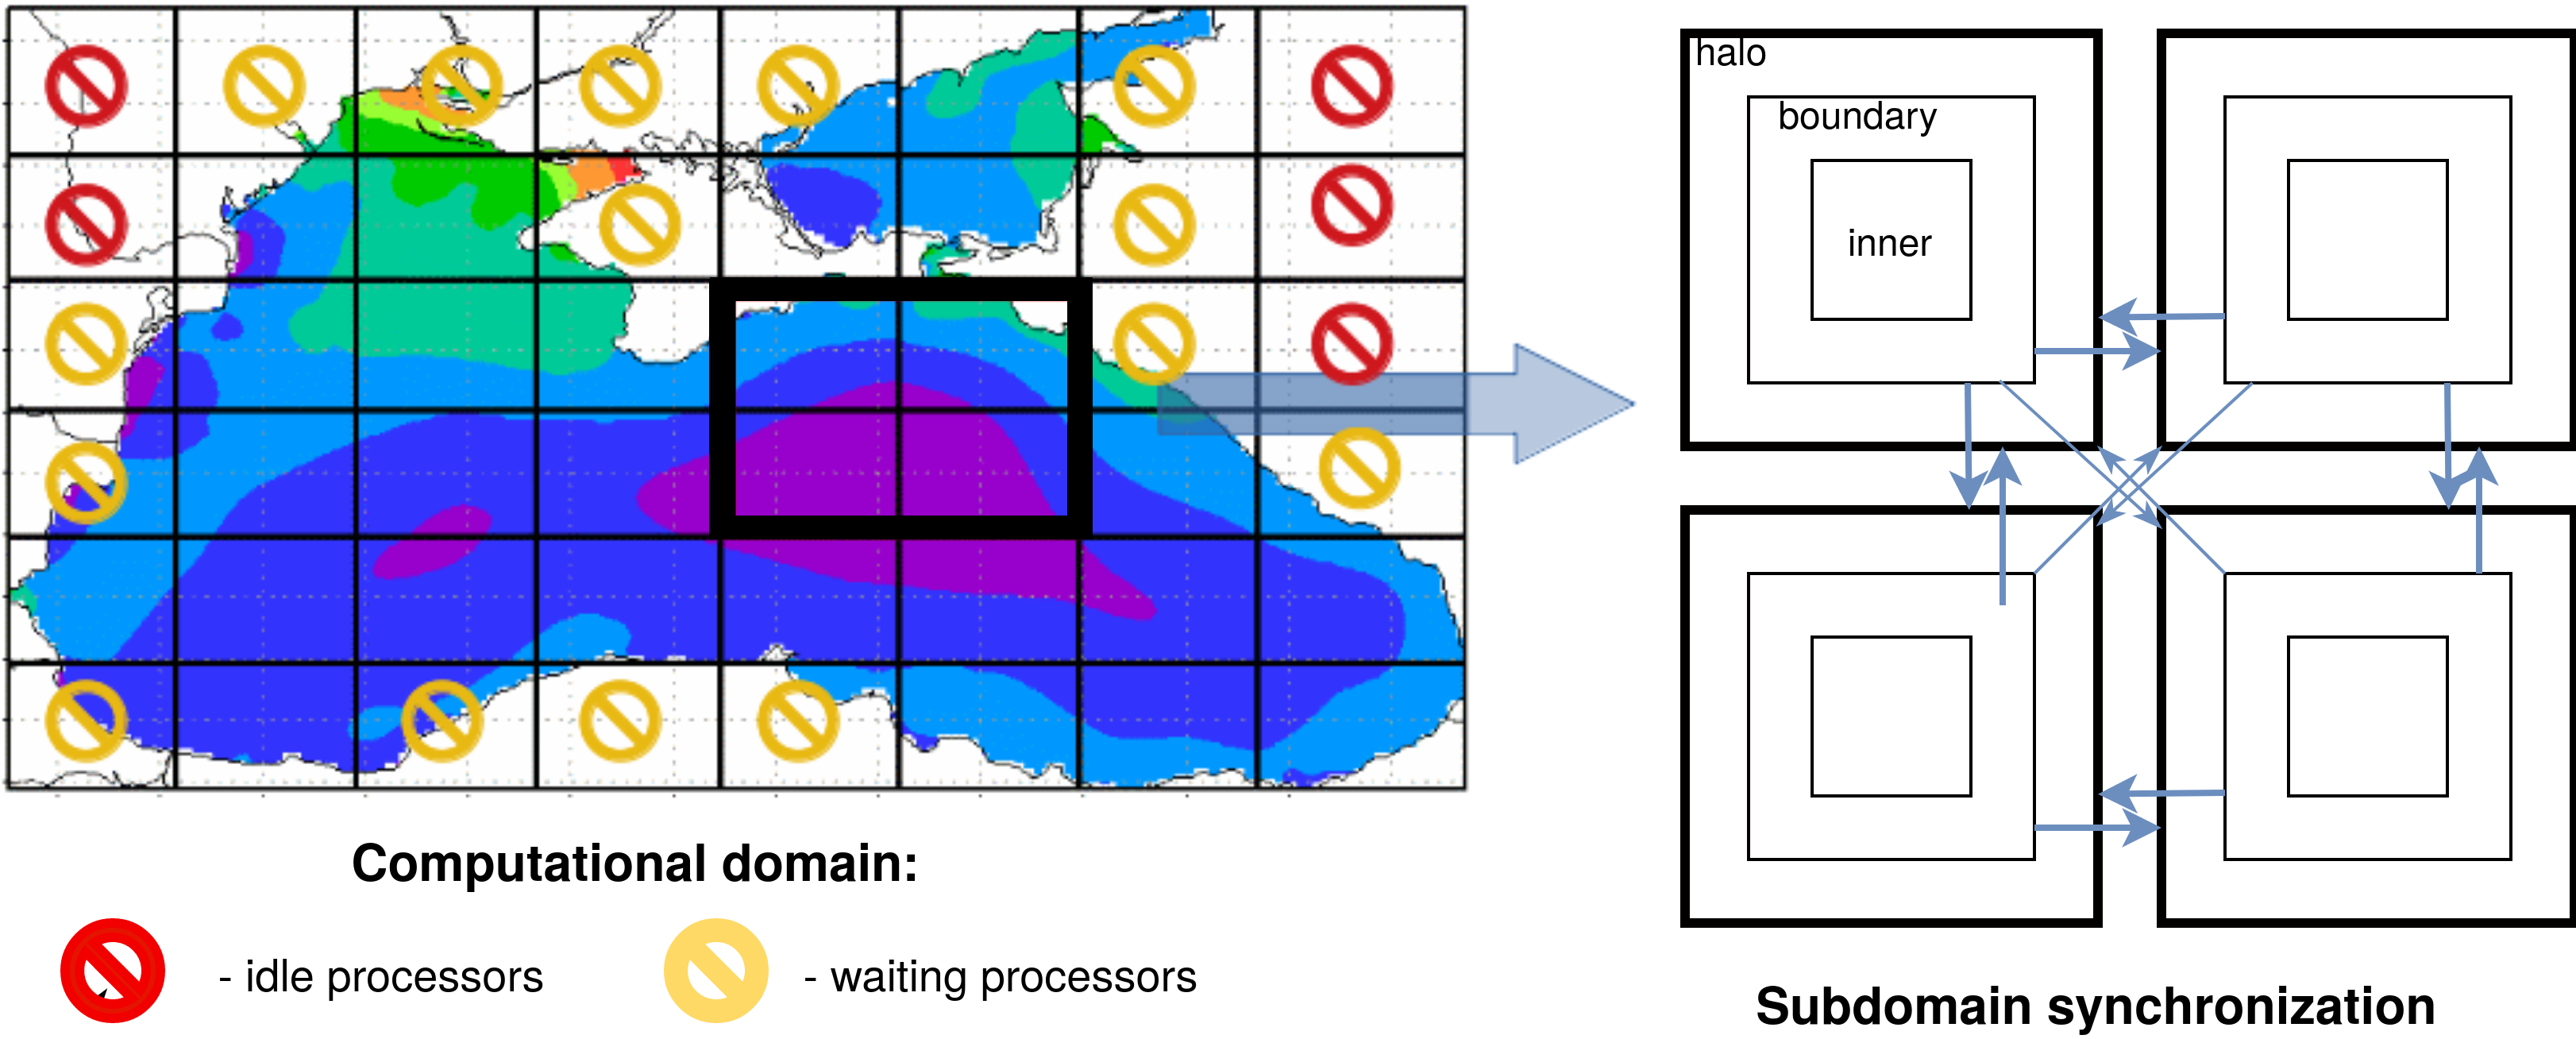
\includegraphics[scale = 0.75]{DDM.png}
    \caption{Слева: равномерное разбиение на прямоугольные подобласти, красным помечены подобласти, попадающие полностью на сушу;
    желтым помечены подобласти, загруженные менее чем на половину. Справа: механизм синхронизаций, красным показана граница каждой подобласти,
    синим показана внерасчетная граница и зеленым помечены внутренние точки подобласти.}
    \label{fig:ddm}
\end{figure}

Наиболее распространенным и легко реализуемым методом разбиения на подобласти является метод равномерного разбиения на прямоугольные подобласти,
этот метод и механизм синхронизаций представлены на рис. \ref{fig:ddm}. На рис. \ref{fig:ddm} также видно,
что из-за неоднородности акватории при таком разбиении часть подобластей полностью попадает на сушу и не участвует в вычислениях,
а часть загружена менее чем на половину из-за большого количества точек суши внутри подобластей.
При таком подходе выходит, что часть процессоров простаивает в вычислениях,
а другая часть часто находится в ожидании из-за недостаточной загруженности.

Поэтому в модели был реализован усовершенствованный метод разбиения на подобасти, так называемый блочный подход.
Суть этого подхода в следующем: исходная расчетная область равномерно разбивается на прямоугольные блоки малого размера,
и каждому процессору ставится в соответствие некоторый набор блоков, которые и формируют его расчётную подобласть, пример показан на рис. \ref{fig:LBalgo}.
Все вычисления в модели происходят по блокам, у каждого блока есть своя внерасчетная граница. Если блоки находятся внутри одной подобластии,
то при синхронизации происходит обычное копирование границы блока на внерасчетную границу соседнего блока. Если блоки находятся на соседних подоблостях,
то при синхронизации используется по-прежнему технология MPI.
Блочный подход уже успел зарекомендовать себя в таких моделях океана, как Parallel Ocean Program (POP) \cite{POP}, \cite{gmd-7-267-2014} и
HIROMB (High Resolution Operational Model for the Baltic Sea) \cite{HIROMB}.


Рассматриваемый блочный подход имеет ряд преимуществ:
\begin{itemize}
    \item Подобласти могут быть произвольными многоугольниками. Действительно, т.к. подобласть состоит из набора блоков малого размера, то можно формировать подобласти довольно произвольной формы. Это свойство позволяет проводить метод балансировки нагрузки вычислений на процессоры, формируя подобласти примерно одинаковой загруженности, о чем будет более подробно написано в следующем разделе.
    \item Эффективная работа с кэш памятью. Выбирая блок малого размера, можно получить прирост в производительности за счет эффективной работы с памятью.
    Для гидродинамических моделей это свойство крайне важно, т.к. любое вычисление на сетке сопровождается большим количеством обращений в память.
    Если блоки, для которых проводятся вычисления, помещаются полностью в кэш память, то  многочисленные обращения в память перестают быть такими дорогостоящими,
    и можно ожидать значительный прирост в производительности.
\end{itemize}

Также блочный подход имеет недостаток:
\begin{itemize}
    \item Дополнительные затраты на копирование внерасчетной границы блоков при синхронизации.
\end{itemize}

В разделе с вычислительными экспериментами будет показано, что при малом размере блоков эффективная работа с кэш памятью компенсирует затраты на копирование при синхронизации, и поэтому этот недостаток можно считать не таким существенным.

\section{Метод балансировки нагрузки вычислений}\label{sec:ch2/sec3}

Под балансировкой нагрузки вычислений имеется в виду такое распределение подзадач между процессорами, 
которое обеспечивает наиболее равномерно распределенную нагрузку на процессоры и минимальные затраты на передачу данных между ними.
Методы балансировки нагрузки вычислений позволяют снизить время простоя отдельных процессоров
и тем самым повысить эффективность параллельной программы, что существенно важно при решении задач 
на высокопроизводительных вычислительных системах.
Балансировка нагрузки вычислений особенно актуальна в задачах моделирования циркуляции океана и моделирования цунами,
потому что из-за наличия берегов и островов в этих задачах равномерное разбиение будет давать особенно несбалансированные подобласти, как будет показано далее в работе.
Тут важно отметить, что оптимальность разбиения для мелкой воды будет точно соответствовать оптимальности для трехмерной сигма-модели INMOM, 
так как количество расчетных уровней по глубине в сигма-модели одинаково для всех точек сетки по горизонтали. 

Существуют два основных способа балансировки нагрузки: методы, основанные на графах, и геометрические методы. 
Методы, основанные на графах, реализованы, например, в библиотеках METIS и parMETIS \cite{METIS} и пользуются довольно большой популярностью. 
Такие методы представляют расчётную область в виде графа, в котором вершины соответствуют узлам сетки, а рёбра - связям между узлами.
Однако у них есть недостаток - это их сложность для программной реализации. 
Поэтому, как альтернатива этим методам, в задачах моделирования океана часто используются 
геометрические методы, такие как разбиение вдоль фрактальной кривой \cite{Dennis2007}, рекурсивной бисекции \cite{Rantakokko1998} и др. 
Такие методы основаны на том, что каждый узел имеет связи со своими соседями.
Геометрические методы дают разбиение хорошего качества и это хорошая альтернатива METIS/parMETIS для многих задач. 
    
В данной работе рассматривается один из геометрических методов балансировки нагрузки: метод разбиения вдоль фрактальной кривой, который
уже успел зарекомендовать себя во многих работах, например, в \cite{Dennis2007}, \cite{Hui2017}. 

В работе показано, что данный метод показывает хорошие результаты применительно к решению уравнений мелкой воды, а также показано сравнение этого метода с METIS.

\subsection{Метод разбиения вдоль фрактальной кривой}

Метод разбиения вдоль фрактальной кривой основывается на фрактальных кривых заполняющих пространство (Space-Filling Curve, SFC).
Такие кривые преобразуют d-мерное пространство в одномерное с сохранением свойства локальности,
т.е. соседние элементы в d-мерном пространстве преобразуются в соседние элементы в одномерном пространстве.
Существует целое множество кривых, заполняющих пространство \cite{SFC1994}. 
На практике используются кривые Пеано и их частные случаи - кривые Гильберта и кривые Мортона \cite{Dennis2007}, \cite{Hui2017}, \cite{gmd-7-267-2014}.
В рамках применения метода разбиения вдоль фрактальной кривой к решению нелинейных уравнений мелкой воды, 
в данной работе будут рассматриваться кривые Гильберта в двумерном пространстве.
    
Кривые Гильберта используются для преобразования двумерной области с размерами $nb_x \times nb_y$ в кривую, где
$nb_x \times nb_y = 2^n$ и $n$ - это целое число, которое называется индексом кривой Гильберта.
Рис. \ref{fig:HC} показывает пример кривых Гильберта с индексами 2, 4, 8.
    
    \begin{figure}[htb!]
    \begin{minipage}[h]{0.3\linewidth}
    \center{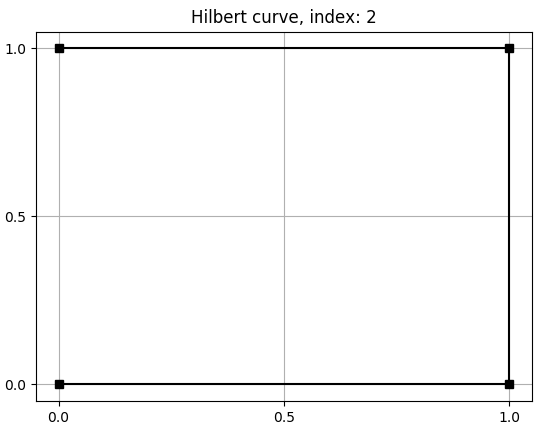
\includegraphics[scale = 0.4]{HC_index2.png}}
    \end{minipage}
    \hfill
    \begin{minipage}[h]{0.3\linewidth}
    \center{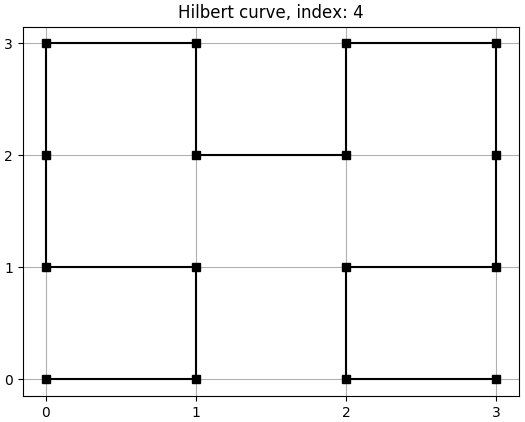
\includegraphics[scale = 0.4]{HC_index4.png}}
    \end{minipage}
    \hfill
    \begin{minipage}[h]{0.3\linewidth}
    \center{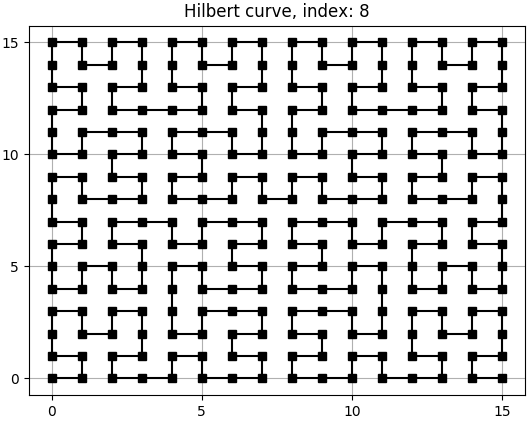
\includegraphics[scale = 0.4]{HC_index8.png}}
    \end{minipage}
    \caption{Кривые Гильберта с индексами 2, 4 и 8 соответственно}
    \label{fig:HC}
    \end{figure}
    
Алгоритм балансировки нагрузки с помощью кривых Гильберта следующий. 
Предварительно вся расчётная область с размерами $nx \times ny$ точек равномерно разбивается
на сетку с размерами $nb_x \times nb_y = 2^n$, состоящую из прямоугольных блоков.
Для каждого блока рассчитывается значение загруженности блока $w_i$ как сумма всех точек, которые не лежат на суше.
Далее, на сетке блоков проводится кривая Гильберта, которая переводит
двумерное пространство блоков в одномерное.
Разбиение на подобласти происходит вдоль кривой и причем таким образом, чтобы
подобласти имели примерно одинаковую сумму загруженности блоков.
Затем каждому процессору ставится в соответствие его подобласть, на которой он проводит вычисления.
Блоки, которые полностью состоят из точек на суше (т.е. загруженность которых $w_i = 0$),
в распределении по процессорам и в дальнейших вычислениях не участвуют. 
На рис. \ref{fig:LBalgo} наглядно показаны шаги описанного алгоритма. 

    
    \begin{figure}[htb!]
    \begin{minipage}[h]{0.32\linewidth}
    \center{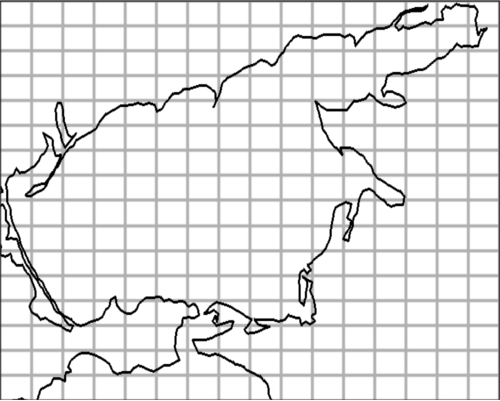
\includegraphics[width=1.0\linewidth, height=140pt]{blockgrid.png}}
    \end{minipage}
    \hfill
    \begin{minipage}[h]{0.32\linewidth}
    \center{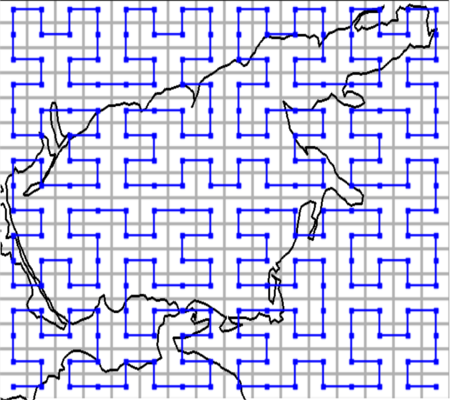
\includegraphics[width=1.0\linewidth, height=140pt]{blockhilbert.png}}
    \end{minipage}
    \hfill
    \begin{minipage}[h]{0.32\linewidth}
    \center{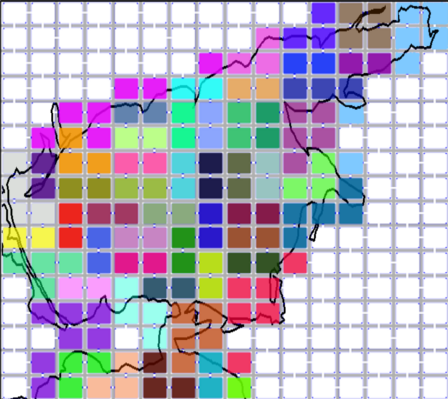
\includegraphics[width=1.0\linewidth, height=140pt]{hilbertLB.png}}
    \end{minipage}
    \caption{Алгоритм балансировки нагрузки с помощью кривых Гильберта. 1) Равномерное разбиение на блоки 
             2) На сетке блоков проводится кривая Гильберта
             3) Блоки объединяются в подобласти вдоль кривой Гильберта.
                Каждому процессору ставится в соответствие его подобласть. }
    \label{fig:LBalgo}
    \end{figure}
    
    
Пример такого разбиения в сравнении с равномерным разбиением без балансировки нагрузки и с разбиением, полученным с помощью библиотеки METIS,
приведён на рис. \ref{fig:map_uniform_hilbert_metis} для акватории Азовского моря с размерами $1525 \times 1115$ точек, 
сетка блоков $32 \times 32$.
Чёрным цветом на рисунке изображены блоки, состоящие только из точек на суше и которые не
участвуют в вычислениях.
    
    \begin{figure}[htb!]
    \begin{minipage}[h]{0.32\linewidth}
    \center{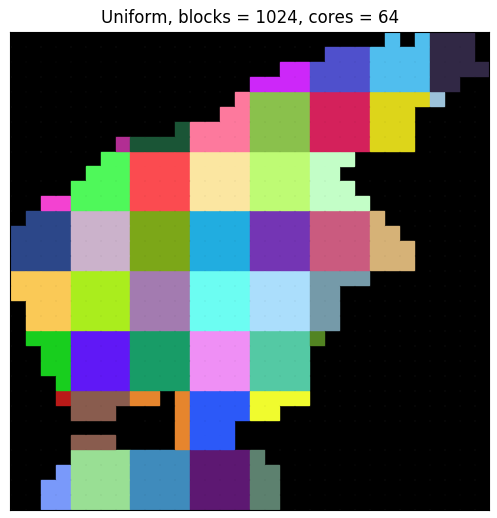
\includegraphics[width=1.0\linewidth]{1024b_64p_u.png}}
    \end{minipage}
    \hfill
    \begin{minipage}[h]{0.32\linewidth}
    \center{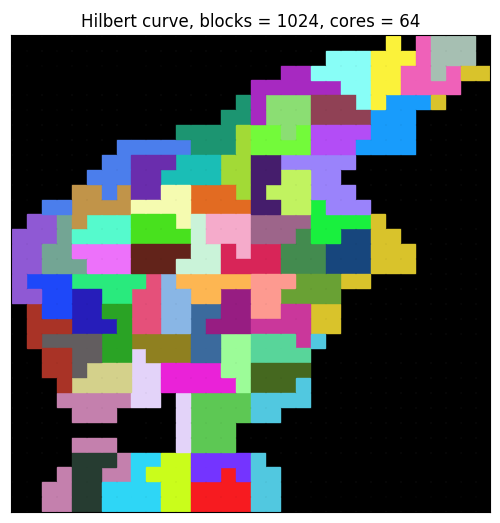
\includegraphics[width=1.0\linewidth]{1024b_64p_h.png}}
    \end{minipage}
    \hfill
    \begin{minipage}[h]{0.32\linewidth}
    \center{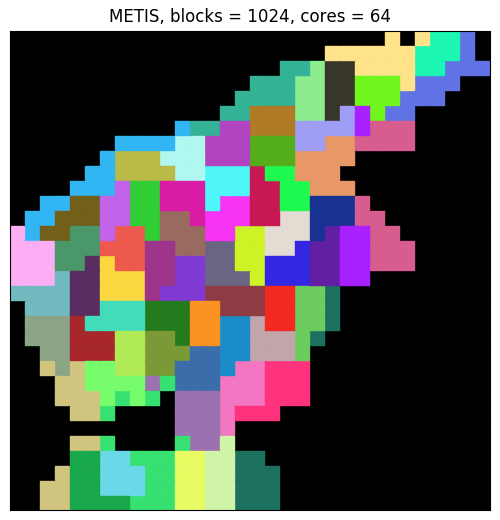
\includegraphics[width=1.0\linewidth]{1024b_64p_metis.png}}
    \end{minipage}
    \caption{Различные разбиения для 64 процессоров, 1024 блоков. 1) Равномерное разбиение 2) Метод разбиения c использованием кривой Гильберта 
             3) Разбиение полученное с помощью METIS}
    \label{fig:map_uniform_hilbert_metis}
    \end{figure}
    
Следует отметить, что у описанного метода балансировки нагрузки вычислений с использованием кривых Гильберта есть несколько недостатков:
ограничение на сетку блоков (сетка должна быть размерами $nb_x \times nb_y = 2^n$); 
большое количество пересылок при большом количестве блоков на процессоре.

\subsection{Метрики качества разбиения}
\label{sec:ch2/sec3/lb}

Для того, чтобы понимать качество полученного разбиения, полезно иметь некоторые метрики \cite{Dennis2007}, \cite{Hui2017}.
В этой части мы введем пару метрик качества разбиения. Предположим, что разбиение происходит на $k$ подобластей для $p$ процессоров.
Введём первую метрику $LB$, которая будет отвечать за сбалансированность разбиения с точки зрения нагрузки вычислений на процессоры:

\begin{equation} \label{eq:LB}  
    \displaystyle { LB = \frac{\max_{1 \leq i \leq k} W_i}{\frac{1}{p}\sum_{i=1}^k W_i} }
\end{equation} 

где $\max_{1 \leq i \leq k} W_i$ - максимальная загруженность $i$ подобласти, $\sum_{i=1}^k W_i$ - полная загруженность всей расчётной области.
Эта величина показывает отношение максимальной загруженности подобласти в разбиении к оптимальной загруженности.
Значение $LB = 1$ соответствует идеально сбалансированному разбиению. 
    % (с точки зрения нагрузки вычислений на процессоры)
    
Введём также вторую метрику $r_M$, которая будет отвечать за качество разбиения с точки зрения коммуникаций между соседними подобластями:

\begin{equation} \label{eq:RM}  
    \displaystyle { r_M = max_{1 \leq i \leq k} \frac{e_i}{s_i} }
\end{equation} 

где $e_i$ - количество узлов $i$ подобласти, которые соседние для некоторой другой подобласти, $s_i$ - количество всех узлов $i$ подобласти.
Эта величина показывает максимальное отношение периметра к объему подобласти. 
Для разбиений с завышенной величиной $r_M$ время на коммуникации между процессорами становится доминирующим.
%Чем это отношение меньше - тем происходит меньше коммуникаций и больше вычислений для подобласти. 
Библиотека METIS по умолчанию пытается построить разбиение, минимизирующее именно такую метрику.
   
Было проведено сравнение метода балансировки нагрузки вычислений, использующего кривую Гильберта, с библиотекой METIS.
В таблице \ref{tab:LB} приведены метрики качеств полученных разбиений. 
На рис. \ref{fig:map_uniform_hilbert_metis} показаны разбиения для 64 ядер. 
Методы рассматривались на сетках блоков: по 8 блоков на ядро для 32 и 128 ядер и по 16 блоков на ядро для всех остальных. 
Видно, что метод балансировки с использованием кривых Гильберта даёт разбиения, очень близкие к разбиениям METIS, как по значениям метрик качества разбиения, так и по значениям полученного ускорения параллельной программы.    
Для 256 ядер видно даже, что по всем метрикам качества разбиение, полученное с помощью кривых Гильберта, немного лучше чем METIS.
Поэтому можно сделать вывод, что для данной задачи метод балансировки нагрузки вычислений с использованием кривой Гильберта - это хорошая альтернатива библиотеке METIS.   
    
%В целом, для рассмотренной задачи выяснилось, что можно использовать как балансировку нагрузки с использованием кривых Гильберта так и METIS. 
Отметим, что метод балансировки с использованием кривых Гильберта строит разбиения в несколько раз быстрее METIS, но для рассматриваемой задачи это незначительно, т.к. расчетное время на порядок больше чем время построения разбиения. 
Однако, алгоритм балансировки с использованием кривых Гильберта будет давать существенные преимущества по сравнению с METIS, когда задача будет упираться во время построения разбиения, например, на очень большой расчетной области и с адаптивной сеткой.
Также описанный алгоритм балансировки предпочтительнее чем METIS, так как он реализован непосредственно в модели и его реализация довольно простая в отличие от того, что реализовано в METIS. METIS - это библиотека для разбиений вообще произвольного вида, в ней реализованы довольно громоздкие методы, основанные на графах. А балансировка с использованием кривых Гильберта - это геометрический метод, который сильно проще и очень хорошо подходит именно для рассматриваемой задачи.  
Используя описанный алгоритм балансировки нагрузки, у модели не будет привязки к сторонней библиотеке, поэтому дальнейшая разработка, поддержка и улучшения этого инструмента будут легче чем работа с METIS.
    
%Из рисунка видно, что оптимальной сеткой блоков для данной задачи является сетка с размерами $32 \times 32$.
%При такой сетке для данной задачи размер каждого блока составляет 1660 точек.
%Ухудшение масштабируемости для сетки блоков с размерами $64 \times 64$ можно объяснить тем, что
%при таком большом количестве блоков коммуникационные задержки на перессылки между блоками
%становятся существенными, хоть и подобласти при таком разбиении будут более сбалансированными (см. таблицу).
    
\begin{table}[]
    \caption{a) Метрика $LB$ для различных разбиений b) Метрика $r_M$ для различных разбиений}\label{tab:LB}
    \begin{subtable}{.5\linewidth}
    \centering
    \caption{}
    \resizebox{0.9\textwidth}{!}
    {
    \begin{tabular}{|l|l|l|l|l|l|}
    \hline
    Cores     & 4      & 16     & 64     & 128    & 256    \\ 
    \hline
    Blocks 
    per core  & 16     & 16     & 16     & 8      & 16     \\
    \hline
    Uniform   & 1.5278 & 2.3872 & 2.4025 & 2.4025 & 2.4025 \\
    \hline
    Hilbert   & 1.0535 & 1.0655 & 1.0640 & 1.2012 & 1.0651 \\
    \hline
    METIS     & 1.0384 & 1.0511 & 1.1080 & 1.1714 & 1.1006 \\
    \hline
    \end{tabular}
    }
    \end{subtable}
    \begin{subtable}{.5\linewidth}
    \centering
    \caption{}
    \resizebox{0.92\textwidth}{!}
    {
	\begin{tabular}{|l|l|l|l|l|l|}
    \hline
    Cores     & 4       & 16      & 64      & 128     & 256     \\ 
    \hline
    Blocks 
    per core  & 16      & 16      & 16      & 8       & 16      \\
    \hline
    Uniform   & 0.311\% & 1.248\% & 2.501\% & 3.554\% & 5.003\% \\
    \hline
    Hilbert   & 1.279\% & 2.558\% & 5.417\% & 7.300\% & 10.88\% \\
    \hline
    METIS     & 0.716\% & 2.501\% & 5.185\% & 8.719\% & 12.13\% \\
    \hline
    \end{tabular}
    }
    \end{subtable}
\end{table}

\section{Гибридная модель параллельного программирования для использования на многопроцессорных системах}\label{sec:ch2/sec4}

Гибридные модели, сочетающие в себе технологии передачи сообщений MPI для архитектур с распределенной памятью и многопоточной обработки данных OpenMP для архитектур с общей памятью, становятся все более популярными, поскольку современные высокопроизводительные вычислительные системы представляют собой набор многопроцессорных систем с общей памятью (вычислительных узлов), объединенных в единую коммуникационную сеть. 
Создание моделей, эффективно использующих ресурсы таких вычислительных систем, является актуальной задачей на сегодняшний день \cite{gmd-11-1799-2018}.
	    
Узкое место в рассматриваемой модели мелкой воды - это синхронизации MPI между процессорами, т.к.  при увеличении числа вычислительных узлов возрастают накладные расходы на синхронизации из-за высокой нагрузки на сеть. Можно уменьшить синхронизации, и тем самым уменьшить нагрузку на сеть, если использовать OpenMP для распараллеливания на общей памяти внутри узла. Это так называемый гибридный подход. Если при использовании только технологии MPI, в так называемом чистом MPI подходе, для каждого ядра на узле создается отдельный MPI процесс, то в гибридном MPI + OpenMP подходе на каждый узел создается только один MPI процесс, и для каждого ядра создаются отдельные потоки. Гибридные подходы в последнее время становятся все более актуальными и используются во многих гидродинамических моделях \cite{Liu2019ParallelIA}, \cite{Afzal_Ansari_Faizabadi_Ramis_2016}, \cite{MPIOpenMP2017},  \cite{Mortikov2016}.

	\begin{figure}[htb!]
    \center
    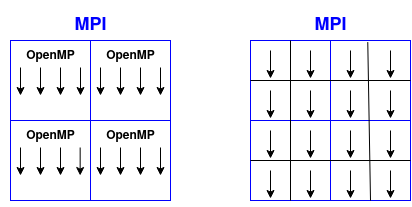
\includegraphics[scale = 0.5]{openmp.png}
    \caption{Гибридные MPI + OpenMP подходы. Слева векторный подход; справа задачный подход.}
    \label{fig:openmp}
    \end{figure}

Есть два подхода при использовании технологии OpenMP для распараллеливания на общей памяти \cite{Wellein2003}. Первый и наиболее распространенный подход называется векторным подходом (vector based). При этом подходе происходит распараллеливание по потокам всех вычислений в модели по подобласти, как схематично показано слева на рис. \ref{fig:openmp}. Т.е. каждому MPI процессу соответствует некоторая подобласть, и все OpenMP потоки существуют и проводят вычисления внутри этой общей для них подобласти. Этот подход легко реализуем, но демонстрирует малую производительность во многом из-за того, что потоки OpenMP неэффективно используют кэш память при работе на общей памяти.

Второй подход называется задачным подходом (task based). Главная идея в этом подходе заключается в том, чтобы использовать метод декомпозиции области для потоков OpenMP, т.е. ставить каждому потоку в соответствие некоторую подобласть. При таком подходе каждый поток существует и проводит вычисления на своей собственной подобласти, как схематично показано справа на рис. \ref{fig:openmp}. За основу гибридного MPI + OpenMP подхода в модели мелкой воды был взят именно задачный подход. Блоки из разбиения распределяются как по процессам MPI, так и по потокам OpenMP. Распределение блоков по MPI процессам происходит с использованием метода балансировки нагрузки вычислений, описанного в предыдущем разделе, и далее происходит распределение блоков по OpenMP потокам внутри каждого MPI процесса с использованием жадного алгоритма следующим образом: все доступные блоки MPI процесса сортируются по величине загруженности и далее в этом порядке по одному распределяются на все доступные потоки внутри MPI процесса. Такой алгоритм, при условии, что количество блоков в разбиении велико, обеспечивает равномерную нагрузку вычислений по всем доступным потокам в вычислительной системе.

В разделе с вычислительными экспериментами будет проведено сравнение двух описанных гибридных подходов MPI + OpenMP и продемонстрировано, что задачный подход во многом эффективнее векторного подхода. Здесь же отметим, что именно задачный OpenMP подход используется в широко известных моделях атмосферы WRF (Weather Research and Forecasting Model) \cite{WRF2016} и океана ROMS (Regional Ocean Modeling System) \cite{Liu2019ParallelIA}, \cite{SHCHEPETKIN2005347}.

Отметим также следующие особенности реализованного гибридного подхода с использованием технологий MPI и OpenMP:

\begin{itemize}
\item У каждого процессора есть буфер для MPI обмена данными c соседними процессорами, в котором имеется место под хранение данных со всех границ блоков подобласти, необходимых для перессылки на соседние процессоры. Синхронизация между подобластями происходит с использованием этого буфера и неблокирующими вызовами MPI, причем синхронизация выполняется одним потоком.

\item При синхронизации копирование границы блоков во внерасчетную границу соседних блоков и в буфер для MPI обмена происходит параллельно всеми потоками OpenMP.

\item Для OpenMP параллельный регион создается в начале запуска модели и существует до конца расчета, что минимизирует временные затраты на инициализацию потоков в модели.
%, как было бы если параллельные регионы создавались и уничтожались динамически в течении расчета модели.

\item Инициализация всех данных происходит в параллельном регионе OpenMP. Это обеспечивает то, что страница памяти выделяется с узла того потока, который первый к ней обратился (first-touch policy). При таком подходе потоки эффективнее работают с памятью в NUMA-системах (Non Uniform Memory Access), в которых доступ в память чужого узла занимает существенно больше времени, чем доступ в память своего узла. 

\item Балансировка нагрузки вычислений по потокам происходит в начале расчета, и далее всюду используется статическое планирование OpenMP потоков по блокам, т.е. используется schedule(static). При динамическом планировании, т.е. при использовании schedule(dynamic), имеются накладные расходы  и происходит менее эффективная работа с памятью, чем при статическом планировании.
 
\item Всюду, где это возможно, используется nowait для параллельных секций OpenMP, чтобы минимизировать точки синхронизации потоков.
\end{itemize}


\section{Гибридные модели параллельного программирования для использования на гетерогенных вычислительных системах}\label{sec:ch2/sec5}

Графические процессоры становятся все более популярными в качестве выбора целевой архитектуры для проведения моделирования климата. 
Имеются примеры успешной адаптации моделей атмосферы и океана для использования на GPU, в том числе моделей мелкой воды \cite{plosSW}, \cite{VOLNA}, \cite{gpuPOM}.

В данной работе, модель мелкой воды была полностью адаптирована для выполнения расчетов на GPU, использую технологию CUDA. 
Было всего адаптировано 15 ядер модели (см. Уровень Ядра модели - раздел \ref{sec:ch2/sec1}) для расчетов на GPU.
Для обеспечения возможности использования различных параллельных шаблонов программирования для вычислений на GPU были произведены модификации в уровне Интерфейс программной архитектуры.
Важно отметить два ключевых аспекта в реализации ядер модели для расчетов на GPU: первым является использование двойной точности во всех вычислениях, а вторым - отсутствие оптимизаций памяти.
Последнее означает, что в ядрах модели не реализованы оптимизации размещения данных на GPU, в частности, не используются общая и текстурная памяти. 
Все обращения к памяти в ядрах модели выполняются непосредственно к глобальной памяти GPU. 
Современные поколения GPU менее чувствительны к оптимизации размещения данных по сравнению с более старыми поколениями, в основном благодаря улучшениям кэшей глобальной памяти, как показано в работе \cite{CUDAopt}.
Авторы данной статьи рассмотрели различные приложения, включая решатель вычислительной гидродинамики, и показали, что использование различных оптимизаций памяти на современных поколениях GPU (Pascal, Volta) в целом не приводит к такому же увеличению производительности, как на более старых поколениях GPU.
Тем не менее, эти результаты следует рассматривать только как часть общей картины. 
Кроме того, мы реализовали ядра модели для вычислений на GPU с минимальными изменениями кода, и адаптацию на GPU можно дополнительно автоматизировать с использованием макросов, как это сделано в работе \cite{gmd-11-3447-2018}.

Реализация на GPU была адаптирована для поддержки блочного подхода в модели мелкой воды, которое успешно использовалось при вычислениях на CPU. 
Благодаря блочному подходу возможно балансирование нагрузки вычислений на GPU.
Было реализовано три параллельных шаблона программирования для вычислений на GPU: синхронный шаблон MPI-CUDA, асинхронный шаблон MPI-OpenMP-CUDA, шаблон MPI-OpenMP-CUDA с использованием нескольких GPU на вычислительном узле.
Эти шаблоны схематично представлены на рисунке \ref{fig:patterns} в сравнении с параллельными шаблонами программирования для вычислений на CPU также реализованными в модели.

\begin{figure}[!ht]
	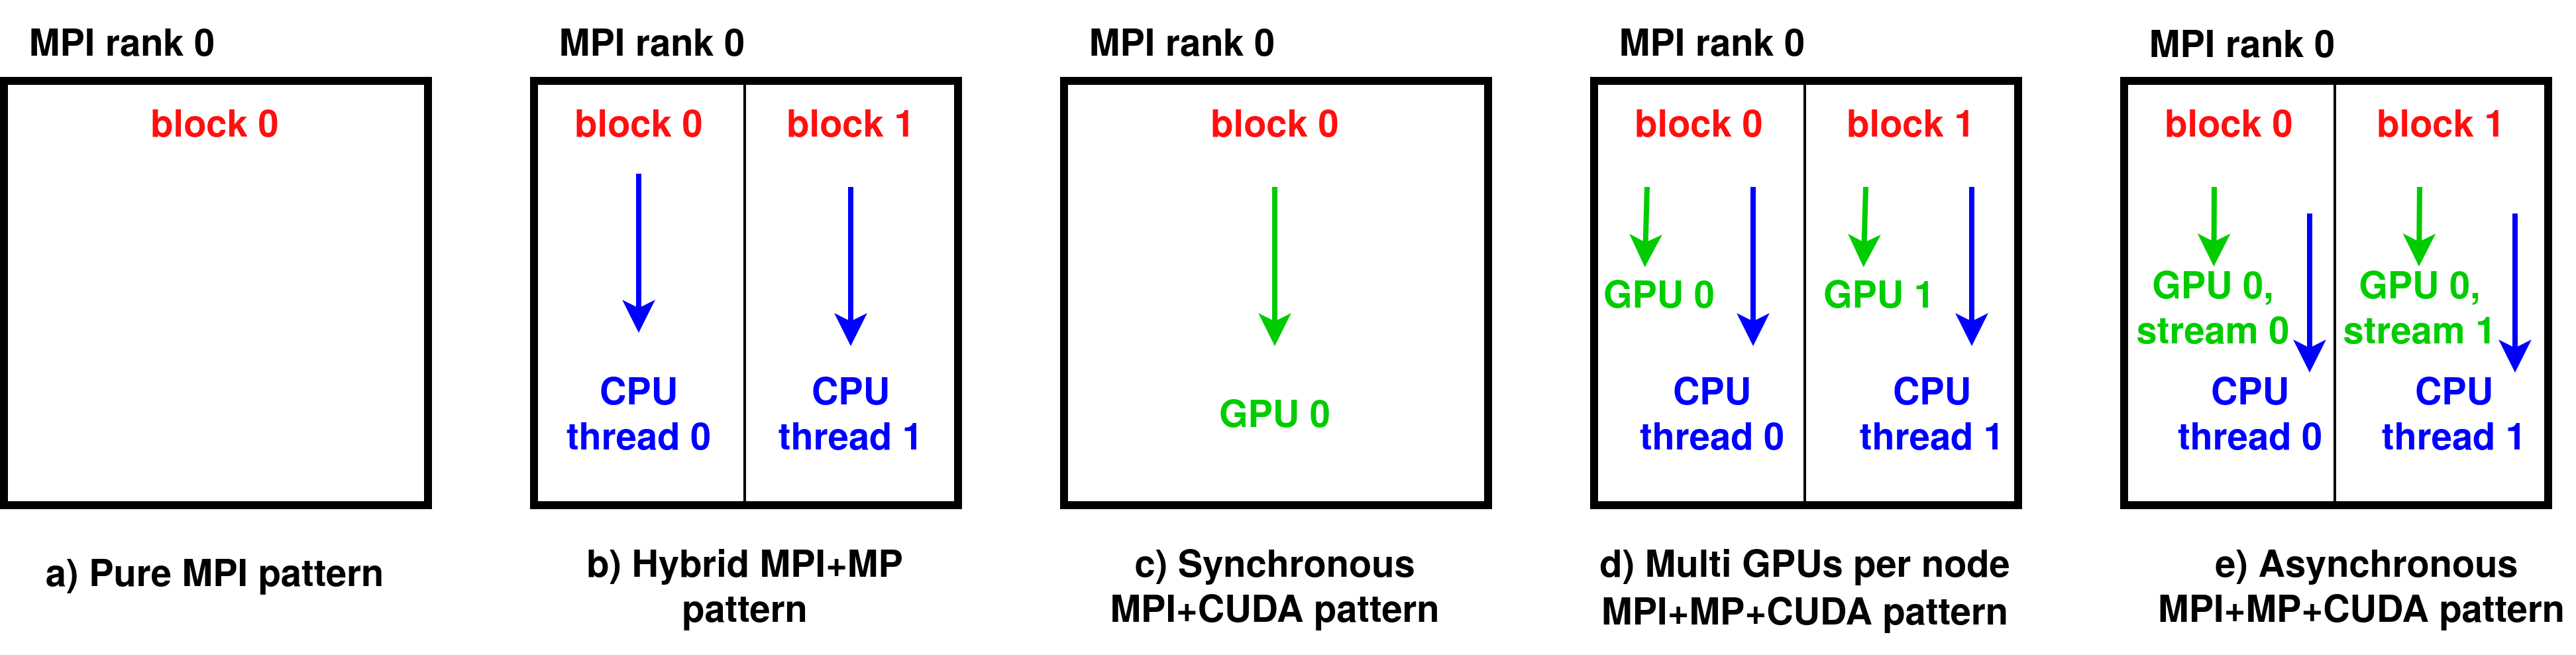
\includegraphics[width=\linewidth]{CPU_GPU_patterns.png}
	\vspace{3pt}
	\caption{Параллельные шаблоны программирования реализованные в модели}
	\label{fig:patterns}
\end{figure}

Обратите внимание, что все эти вычислительные шаблоны не вызывали сложностей при реализации, поскольку архитектура программного обеспечения основана на разделении обязанностей.
Все модификации кода были выполнены на уровне Интерфейс - без модификаций на уровнях Ядро и Алгоритм.
Опишем каждый из параллельных шаблонов программирования для вычислений на GPU более подробно.

\subsubsection{Синхронный шаблон вычислений MPI-CUDA}

В данном подходе каждому процессу MPI назначается подобласть, содержащая только один блок, и один GPU для вычислений, как показано на рисунке \ref{fig:patterns}. 
Вычисления на подобласти выполняются полностью на GPU с использованием технологии CUDA. 
После выполнения вычислений ядра модели на GPU происходит синхронизация процессоров следующим образом:

\begin{enumerate}
\item Граничные точки подобласти синхронно передаются с GPU на CPU, то есть используется блокирующая передача данных.
\item Процессы MPI синхронизируются, и внерасчетная граница каждой подобласти обновляется. Синхронизация MPI выполняется полностью на CPU.
\item Обновленная внерасчетная граница передается обратно с CPU на GPU. Передача данных также синхронная.
\end{enumerate}

Этот шаблон поддерживает вычисления на нескольких GPU, предполагая только один блок и GPU на процесс MPI, и не поддерживает блочный подход. 
Таким образом, в данном подходе отсутствует балансировка нагрузки вычислений на GPU.

\subsubsection{Асинхронный шаблон вычислений MPI-OpenMP-CUDA}

В данном шаблоне поддерживается блочный подход для вычислений на GPU. 
Каждому процессу MPI назначается подобласть, содержащая несколько блоков, и создаются потоки OpenMP и потоки CUDA для каждого блока подобасти в процессе MPI, как показано на рисунке \ref{fig:patterns}. 
Ядро модели запускается для вычислений на GPU для каждого блока подобласти следующим образом:

\begin{enumerate}
\item Каждый поток OpenMP асинхронно запускает ядро модели на GPU для блока подобласти. Запуск выполняется в потоке CUDA, соответствующем потоку OpenMP.
\item Каждый поток OpenMP асинхронно передает граничные точки с GPU на CPU блока подобласти. Передача данных выполняется в потоке CUDA, соответствующем потоку OpenMP.
\item Все потоки CUDA и потоки OpenMP синхронизируются.
\item Процессы MPI синхронизируются, и внерасчетные границы каждого блока подобласти обновляются. Синхронизация MPI выполняется полностью на CPU.
\item Каждый поток OpenMP асинхронно передает обновленные внерасчетные границы с CPU на GPU блока подобласти. Передача данных выполняется в потоке CUDA, соответствующем потоку OpenMP.
\end{enumerate}

Поскольку современные GPU имеют отдельные управляющие элементы для выполнения ядер и передачи данных, этот шаблон вычислений организует асинхронную передачу данных и перекрывает выполнение ядра на GPU с передачей данных между CPU и GPU в разных потоках CUDA. 
На рисунке \ref{fig:GPUpatterns} схематически показаны шаги этого шаблона вычислений сравнительно с синхронным шаблоном MPI-CUDA.
Можно видеть, что передача данных перекрывается с выполнением ядра по времени для асинхронного шаблона MPI-OpenMP-CUDA.
Этот шаблон вычислений полностью гибриден и разработан для более эффективных вычислений на вычислительных узлах с одним GPU на узел по сравнению с синхронным шаблоном MPI-CUDA.

\begin{figure}[!ht]
	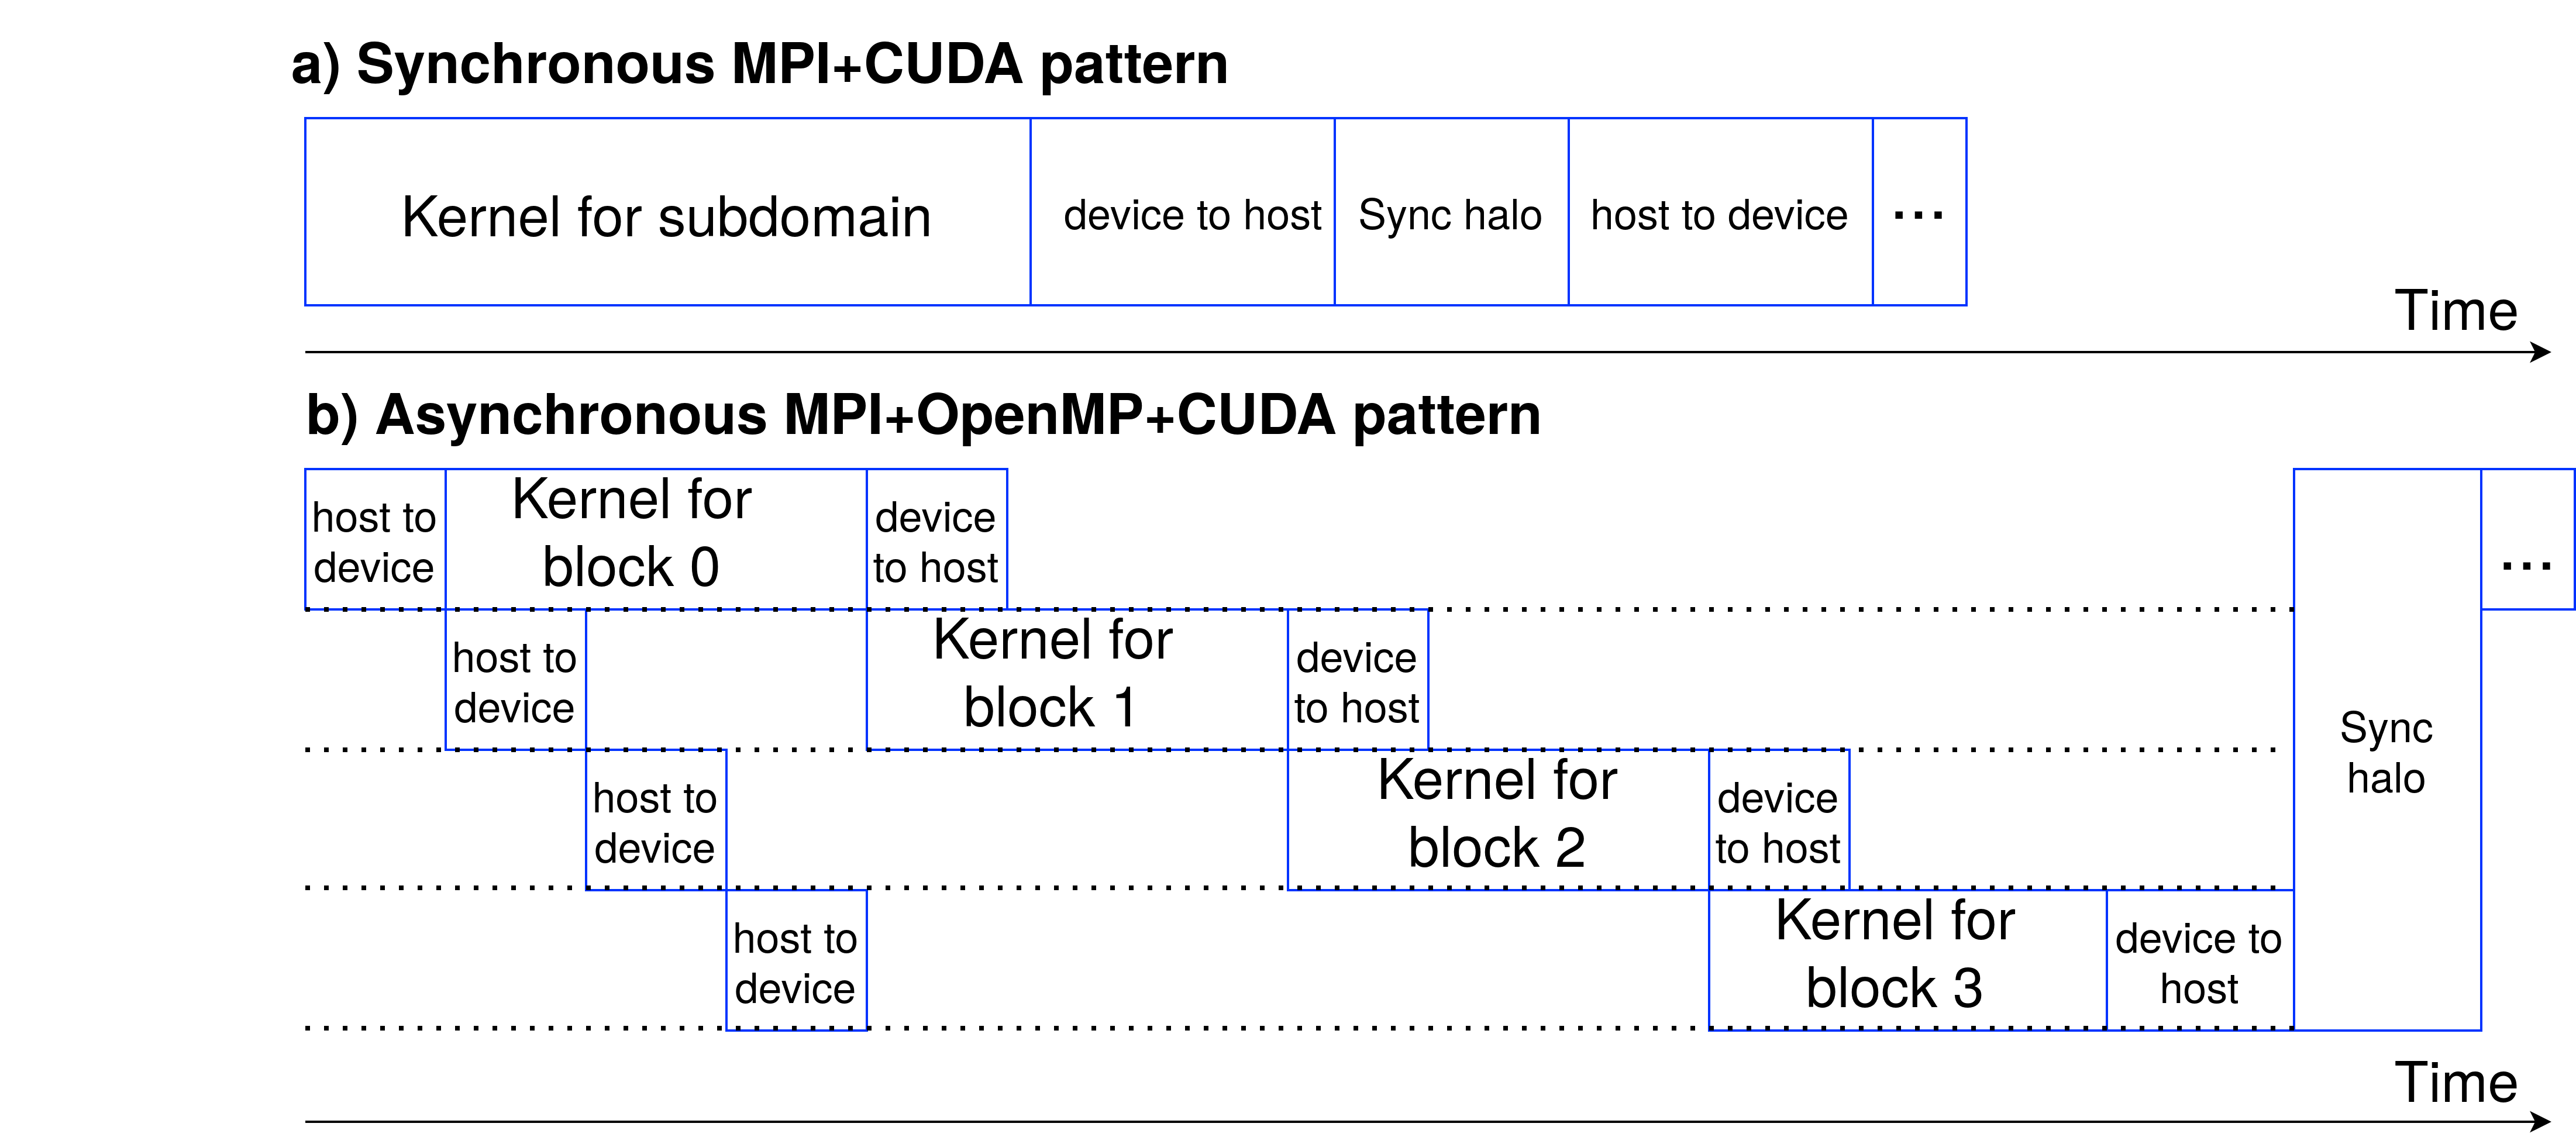
\includegraphics[width=\linewidth]{GPUpatterns.png}
	\vspace{3pt}
	\caption{Синхронный шаблон вычислений MPI-CUDA и асинхронный шаблон вычислений MPI-OpenMP-CUDA}
	\label{fig:GPUpatterns}
\end{figure}

\subsubsection{Шаблон MPI-OpenMP-CUDA с использованием нескольких GPU на вычислительном узле}

Этот шаблон также поддерживает блочный подход для вычислений на GPU, но иначе, чем асинхронный шаблон MPI-OpenMP-CUDA.
Каждому процессу MPI назначается несколько блоков и потоков OpenMP, столько, сколько доступно GPU на узле. 
Следовательно, каждый GPU, управляемый одним потоком OpenMP, содержит один блок подобласти на узле. 
Потоки OpenMP независимо запускают ядра CUDA, что позволяет эффективно использовать каждый доступный GPU на узле. 
Синхронизация организована, как и в шаблоне MPI-CUDA, но с синхронизацией GPU на узле и сбором граничных точек между GPU для синхронизации процессов MPI. Этот подход является полностью гибридным и разработан для вычислений на вычислительных узлах с несколькими GPU на узле.

\FloatBarrier
